\documentclass{article}%
\usepackage[T1]{fontenc}%
\usepackage[utf8]{inputenc}%
\usepackage{lmodern}%
\usepackage{booktabs}%
\usepackage{textcomp}%
\usepackage{lastpage}%
\usepackage{geometry}%
\usepackage{amsmath}%
\geometry{
    paper=a4paper,
    head=0cm,
    left=2cm,
    right=2cm,
    top=0cm,
    bottom=2cm,
    includehead=True,
    includefoot=True
}%
\usepackage{graphicx}%
%
\usepackage{multicol}%
\usepackage{lipsum}%
\usepackage{float}%
\usepackage{verbatim}%
\title{
    Reconstructing Arrival-Times of individual Photons
    in a continous Stream of Night-Sky-Light
}%
\author{Sebastian A. Mueller}%
\date{}%
%
\begin{document}%
\maketitle%

\newcommand{\F}{F_\text{nsb}}
\newcommand{\Ftyp}{F_\text{typical}}
\begin{multicols}{2}%
%
The atmospheric Cherenkov-method can reconstruct the type, energy, and direction of a cosmic particle from the Cherenkov-light emitted in air-showers.
%
Instruments must sense blueish Cherenkov-light, better reject reddish night-sky-light, and must reconstruct the arrival-times of the photons with $\sim{}$5\,ns resolution.
%
Photo-sensors and read-out are cost-drivers of the method.
\newline
%
We expect a continues read-out into digital buffers, where each individual photon is recorded, to be beneficial for the atmospheric Cherenkov-method as it allows fast computational access to all observables.
%
We expect such a read-out to lower the energy-threshold \cite{jung2005star}, to improve the separation of Cherenkov- from night-sky-light, and to improve the reconstruction of the cosmic particle \cite{catalano2008single}.
\newline
%
One way of continues read-out are flash analog-digital-converters (ADC)s.
%
However, their cost and power-consumption scale rapidly with their sampling frequency $f$.
%
\begin{eqnarray*}
\text{Cost} &\sim& f^2,\\
\text{Power} &\sim& f^2.
\end{eqnarray*}
%
In this report, we explore a possible read-out with many slow \mbox{($f$ < 100\,MHz)} ADCs.
%
We want each slow ADC to digitizes the signal of a photo-sensor that have only little acceptances (area and solid angle) and thus a low rate of night-sky-photons.
%
We hope that when the photo-sensor's rate of night-sky-photons is low, a slow ADC in combination with a little computing will be able to reconstruct the arrival-times of the individual photons sufficiently accurate, i.e. better than the sampling period $1/f$.
%
Since the cost of silicon photo-sensors are mostly proportional to their area, there is only little cost overhead when replacing a big sensor with multiple small ones.
%
Due to the rapid scaling of the ADC's demands with sampling frequency $f$, many slow ADCs might outperform fewer fast ADCs in both power-consumption and cost.
\newline
Further, the finer binning of photo-sensors might allow the implementation of small aperture (< 100\,m$^2$) plenoscopes covering large ($> 300\,(1^\circ{})^2$) field-of-views due to computational compensation of optical aberrations. \cite{mueller2019phd}.
%
\section*{Sensing Night-Sky-Photons}%
\label{sec:nsb}%
%
Table \ref{TabFilters} shows the relative yield $\eta_\text{Cer.}$ of Cherenkov-light, and the resulting rate $R_\text{nsb}$ of night-sky-photons for typical photo-sensors.
%
\begin{table}[H]
  \begin{center}
    \begin{tabular}{cccrr}
%
        \footnotesize{sensor} &
        \footnotesize{mirror} &
        \footnotesize{filter} &
        $R_\text{nsb}$ /   &
        $\eta_\text{Cer.}$ / \\
%
        &
        &
        &
        \footnotesize{$10^6\,\text{m}^{-2}\,(1^\circ)^{-2}\,\text{s}^{-1}$} &
        \footnotesize{$10^{-3}$} \\
%
        \hline
        PMT &             &             & 144.8 & 213\\
        .   & $\bullet{}$ &             & 135.8 & 206\\
        .   & $\bullet{}$ & $\bullet{}$ &  15.9 &  53\\
        \hline
        SiPM &             &             & 280.3 & 198\\
        .    & $\bullet{}$ &             & 188.5 & 176\\
        .    & $\bullet{}$ & $\bullet{}$ &   7.1 &  24\\
    \end{tabular}
    \caption{
The rates and yields result out of the typical flux of night-sky-light $\Ftyp{}$, see Figure \ref{fig:nsb}, the sensors detection-efficiencies, see Figure \ref{fig:pde}, and the efficiencies of a  mirror and a filter, see Figure \ref{FigNsbFilter}.
    }
    \label{TabFilters}
  \end{center}
\end{table}
%
The typical flux of night-sky-light corresponds to a sky surface brightness of
%
\begin{eqnarray*}
\Ftyp{} &\hat{=}& 21\,\text{mag}\,\text{arcsec}^{-2}.
\end{eqnarray*}
%
Most observations take place in the range of fluxes from
\begin{eqnarray*}
\approx{}0.8 &> \F{} / \Ftyp{} >& \approx{}3.
\end{eqnarray*}
%
Figure \ref{fig:obstimeFact} shows the distribution of $\F{}$ with a special Cherenkov-telescope FACT which pioneered observations in the brightest full moon conditions using robust silicon photo-sensors.
%
Even with FACT observations beyond $\F{} / \Ftyp{} = 5$ are rare.
%
Table \ref{TabInstrumentsNsbRates} shows the expected rates of night-sky-photons in different instruments.
%
\begin{figure}[H]%
\centering%
\includegraphics[width=1.0\linewidth]{night_sky_background.jpg}%
\caption{
The typical flux $F_\text{Night}$ of night-sky-light \cite{gaug2013night}.
Dotted line is \cite{preuss2002study}.
Gray line is a simulated and arbitrarily scaled Cherenkov-spectrum of a 5\,GeV gamma-ray in Chile at 5\,km a.s.l.
All extrapolated from 700 - 1000\,nm.
}%
\label{fig:nsb}
\end{figure}
%
\begin{figure}[H]%
\centering%
\includegraphics[width=1.0\linewidth]{photon_efficiency.jpg}%
\caption{
Dotted line is silicon-photo-multiplier (SiPM), \mbox{Hamamatsu\,S10362-33-050C}, shape according to \cite{hamamatsu2009mppc}, and scaling according to \cite{anderhub2013design}.
Extrapolated from 700 - 1000\,nm.
Dashed line is photo-multiplier-tube (PMT), \mbox{Hamamatsu\,R11920-100-05} \cite{toyama2013novel}
}%
\label{fig:pde}
\end{figure}
%
\begin{figure}[H]%
\centering%
\includegraphics[width=1.0\linewidth]{nsb_filters.jpg}%
\caption{
Dashed line is CTA's dielectric mirror for the MST, after degrading \cite{pareschi2013status,pareschi2013statusarxiv}.
%
Dotted line is VERITAS' night-sky-filter \cite{archambault2017gamma}.
%
Both Extrapolated from 700\,nm to 1000\,nm.
}%
\label{FigNsbFilter}
\end{figure}
%
\begin{figure}[H]%
\centering%
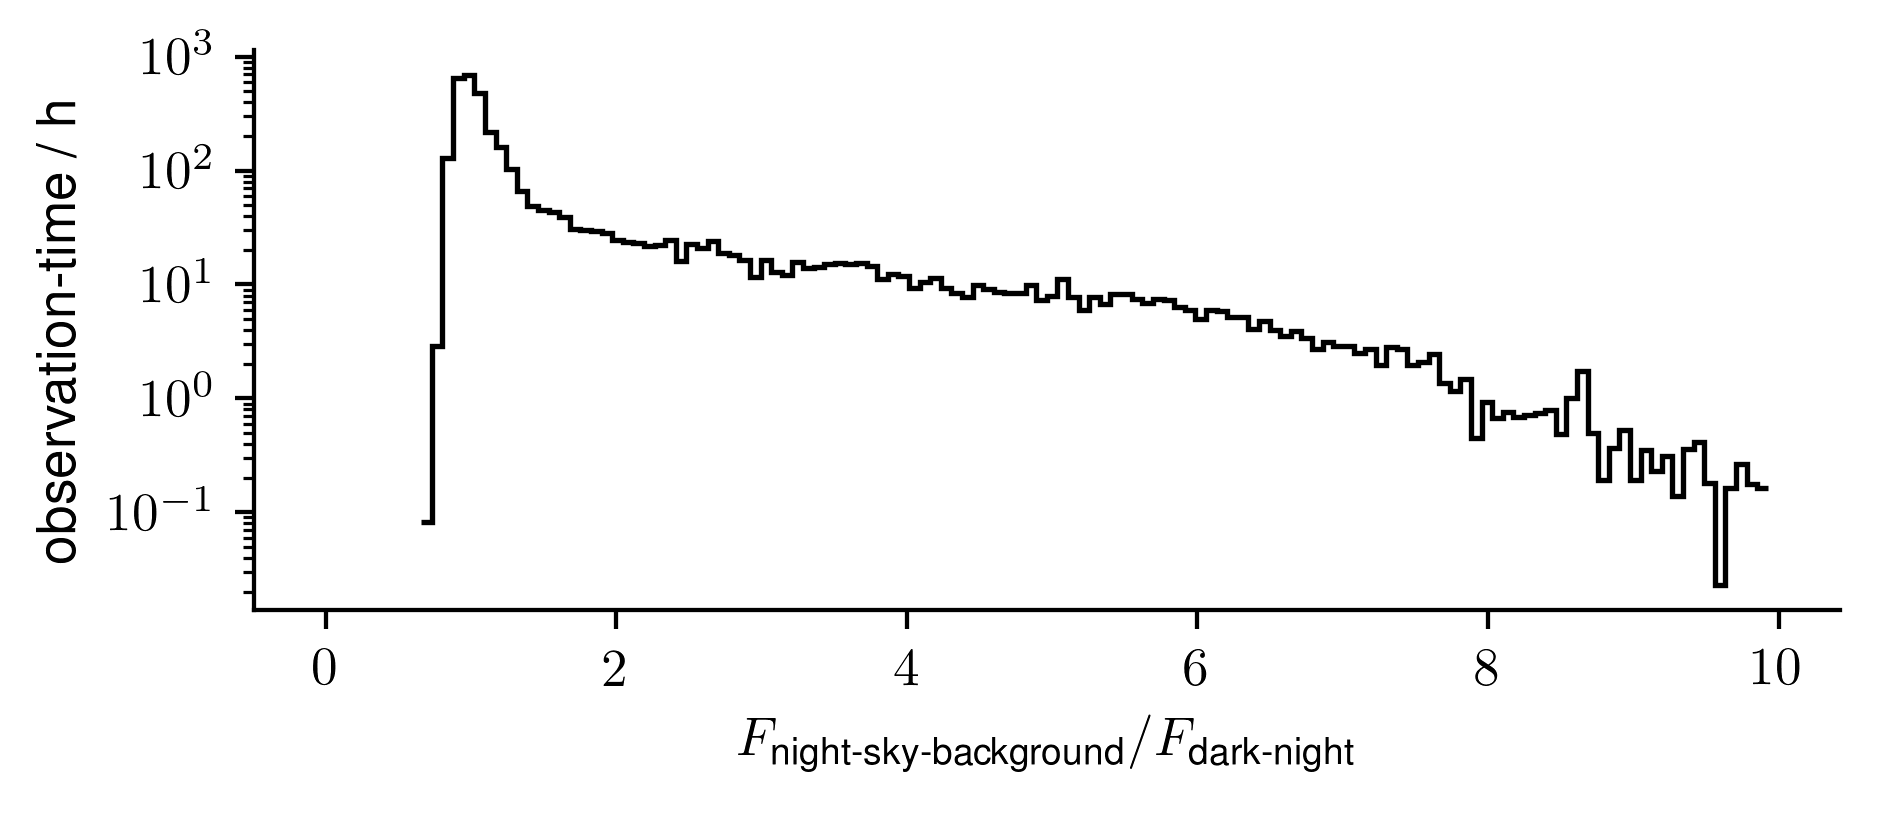
\includegraphics[width=1.0\linewidth]{observation_time_histogram.png}%
\caption{
Figure taken from \cite{mueller2019phd}.
}%
\label{fig:obstimeFact}
\end{figure}
%
\begin{table}[H]
  \begin{center}
    \begin{tabular}{lcrrr}
        &tech.& area/ & fov/&$R$/\\
        &     & m$^2$ & $(1^\circ)^{2}$&$10^6$s$^{-1}$\\
      \hline
      FACT &SiPM& 10 & 0.01 & 29\\
      H.E.S.S. CT-1 &PMT& 108 & 0.0222 & 344\\
      H.E.S.S. CT-5 &PMT& 614 & 0.0039 & 347\\
      Portal, 71m &PMT& 65 & 0.0039 & 37\\
    \end{tabular}
    \caption{Expected rates of night-sky-photons $R$ in an individual read-out-channel (pixel or lixel).}
    \label{TabInstrumentsNsbRates}
  \end{center}
\end{table}
%
\section*{Simulating}%
\label{SecSimulating}%
%
\bibliographystyle{apalike}%
\bibliography{references}%
\end{multicols}{2}%
\end{document}
